\documentclass[12pt]{titlepage} 

\usepackage{fancyhdr} 
\pagestyle{fancy}
\usepackage{amssymb}
\usepackage{caption}
\usepackage{subcaption}
\usepackage{float}
\graphicspath{{Images/}} 
\usepackage[backend=biber,style=phys]{biblatex}
\usepackage{tocbibind}
\usepackage{tabularx}
\usepackage{amsmath}
\usepackage{appendix}
\usepackage{listings}
\usepackage{hyperref}
\addbibresource{references.bib}

\title{Is It Possible to Create a Mathematical Model to Predict Photopollution Based on Population Density in Munster?} 

\author{Conor Casey and Hannah Coombs} 
\college{Teacher: Ms. Abbott} 

\degree{Chemical, Physical, and Mathematical Sciences} 
\degreedate{Stand 3502 - BTYSTE 2019} 

\begin{document}

\maketitle

\clearpage\mbox{}\clearpage

\pagenumbering{roman}

\chapter*{
\centering
    ``Who are we? We find that we live on an insignificant planet of a humdrum star
lost in a galaxy tucked away in some forgotten corner of a universe
in which there are far more galaxies than people.”''
\\[5pt]
\rightline{{\rm --- Carl Sagan}}
}

\chapter*{Comments Page}
\addcontentsline{toc}{chapter}{Comments Page}

\chapter*{Abstract}
\addcontentsline{toc}{chapter}{Abstract}
\section*{Project Aim} 
This project considers the possible relationship between population density and photopollution. Photopollution is light pollution that specifically deals with the visible spectrum of light. This project tests the hypothesis that there is a correlation between population density and photopollution.  

\section*{Experimental Method} 
The experimental method we utilised involved measuring the dark portion of the sky with a telescope and a photometer app. Typically such measurements are made at the zenith: the point at which the sky or celestial sphere is directly above the observer. We collected data at 20 different sites across all the counties of Munster. Once we collected all the data we analysed it in comparison to population density. We got the population, and population density data from the Central Statistics Office website (2016 Census). We used a number of different analysis techniques including the correlation coefficient and standard deviation. We also compared it against an existing model, known as, Walker's Law.  

\section*{Results} 
We found a statistically significant relationship between the independent variable, population density, and the dependent variable, photopollution. This empirical relationship is described by equation \ref{abmodel}. 

\begin{equation} 
\label{abmodel} 
I = 0.03510566 d_x - 14.32414198 
\end{equation} 

In this equation $I$ is the photopollution produced in that area, in the unit of measurement, $LUX$, and $d_x$ is the population density of that area (people per $km^{2}$). There is a correlation coefficient of 0.918 between the two variables. This means there is a strong positive linear correlation between the two variables and that as population density increases, photopollution tends to increase. In comparison, and using the photopollution data we gathered, we found a correlation coefficient of 0.64 in Walker's Law.

\section*{Conclusions and Recommendations} 
Based on our findings, this suggests that population density is a better predictor of  photopollution.  Once we established this empirical relationship, we were able to create a grading system that described what the photopollution value means in relation to stargazing conditions. We used this grading system and mathematical model to develop a Python program, and an app to show the potential practical uses of our findings. Finally, we generated a photopollution map based on our model (see figure \ref{a}) and compared it to a nighttime view of Ireland as provided by the VIIRS 2018 (March) Radiance (see figure \ref{b}). A VIIRS radiance is, nighttime imagery of Planet Earth provided by an instrument board the Suomi NPP satellite (operated by the National Oceanic and Atmospheric Administration) known as the Visible Infrared Imaging Radiometer Suite. The two figures are identical, therefore this proves our model is accurate and could be used by amateur astronomers to paint a better picture of the photopollution in the night sky.

\begin{figure}[h]
    \centering
    \caption{Our generated photopollution map compared against the VIIRS 2018 (March) Radiance}
    \begin{subfigure}{.49\textwidth}
        \centering
        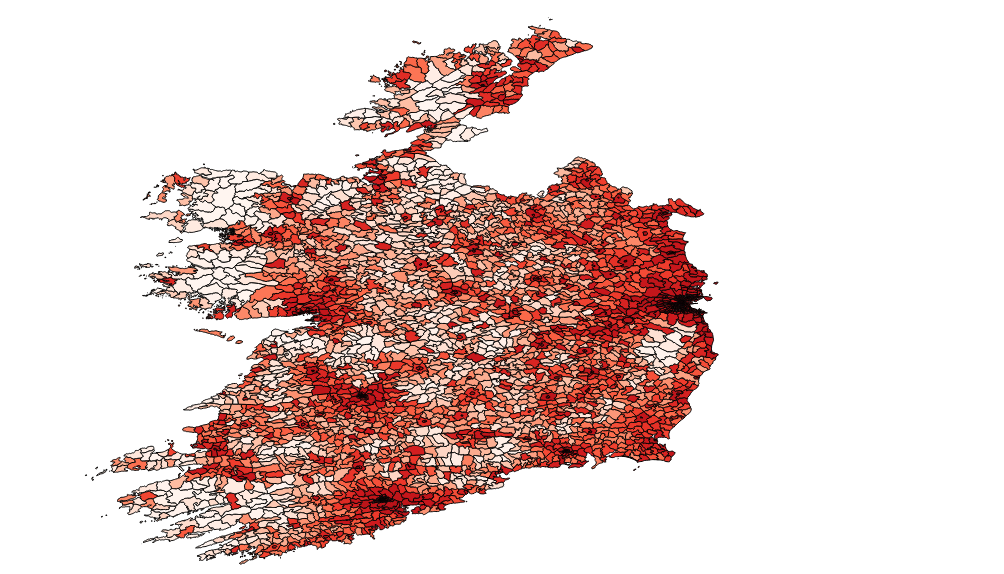
\includegraphics[width=\textwidth]{photopollutionmap}
        \caption{Our generated photopollution map of the Republic of Ireland}
        \label{a}
    \end{subfigure}
    \hfill
    \begin{subfigure}{.49\textwidth}
        \centering
        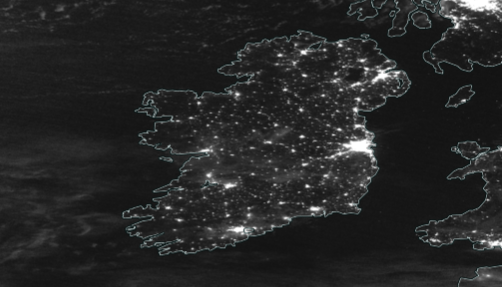
\includegraphics[width=\textwidth]{ireland}
        \caption{Nighttime Imagery of Ireland provided by the VIIRS 2018 (March) Radiance}
        \label{b}
    \end{subfigure}
\end{figure}

\chapter*{Acknowledgements}
\addcontentsline{toc}{chapter}{Acknowledgements}
\paragraph{Ms. Abbott}
First and most importantly, we would like to thank our amazing Science teacher, Miss Abbott. Words cannot begin to express how grateful we both are for her continued support in our project and lives. She's been there for us throughout the last 3 years like no other teacher, always offering us refuge in her classroom. We've been through a lot together in the last few years including some of our happiest times and some of our lowest. She's always been there for us, both academically and personally. 

We want to thank her for the numerous road trips we endured to collect our data. Spending eleven hours with someone in a car is always a struggle, yet, Ms. Abbott never once was annoyed, or frustrated, even when we were at peak sugar rush! Honestly, we are so lucky to have such a giving, kind and funny person in our lives, its even better that she's our teacher and we get to see her almost every day. We would like to thank her for inspiring us to love Science in the first place. 

Speaking as just Conor for a minute, she truly changed the way I view Science as a field in general. I genuinely believe she has changed the course of my life forever. From getting various Physics and Maths books for me, encouraging me to expand what I think I am capable of, and even helping me through the difficult times I am truly grateful; and even though I cannot express how grateful I am in words all the time: THANK YOU SO, SO, SO MUCH! 
\paragraph{Mr. O'Connor}
I would like to thank Mr. O'Connor, my Mathematics teacher, for his help in creating our mathematical model and for assistance in determining what data analysis we should do.
\paragraph{Meg Bevan}
We would like to thank Meg Bevan, of Megabyte Design, for assissting Hannah in the design and production of the poster. Her help is greatly appreciated.
\paragraph{Mr. Healy, and Ms. Foley-Hayes}
I would like to thank Mr. Healy, and Ms. Foley-Hayes, our Principal and Vice Principal, for their support in relation to funding, incorporating various different ideas into our project, and generally providing all the assistance we needed.
\paragraph{Aisling Rochford}
I would like to thank Aisling Rochford, a third year student in our school, for her assistance in developing the Android app we created called “Photopollution Calculator”. It is now available on the Google Play Store for download. 
\paragraph{Brian Harmon}
I would like to thank Brian Harmon for giving up his time on the night of the 18th of November 2018, to drive us to Clare, Limerick and North Kerry. We greatly appreciated the time he committed to this project.
\paragraph{David O'Sullivan}
I would like to thank David O'Sullivan, a former group member and a fellow TY classmate, for his assistance in collecting data over the two separate days. He, unfortunately, had to drop out of this project for unforeseen health circumstances. 
\paragraph{Prof. Brian Espey}
Finally, I would like to thank Brian Espey, professor at TCD, for answering our questions about measuring light pollution, units of measurement, equipment, population density, etc. We would also like to thank him for his guidance in potential future directions of our project. We greatly appreciate his guidance.

\section*{Special thanks to...}
\begin{figure}[H]
    \centering
    
\includegraphics[width=.6\linewidth]{cso}
\end{figure}
\begin{figure}[H]
    \centering
    \begin{subfigure}{.49\linewidth}
        \centering
        
\includegraphics[width=.49\linewidth]{qgsi}
    \end{subfigure}
    \hfill
    \begin{subfigure}{.49\linewidth}
        \centering
        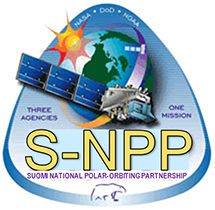
\includegraphics[width=.49\linewidth]{VIIRS}
    \end{subfigure}
\end{figure}

\tableofcontents

\chapter{Introduction} 
\pagenumbering{arabic} 
In this modern world, photopollution data is provided by satellites so as a consequence the idea for this project came to Conor when he was pondering whether it would be possible to determine the severity of photopollution without the need of satellites. Conor was also naturally attracted to Physics and Astronomy as he had a strong proficiency and interest in both. He also lives in Blackwater. Blackwater, is a dark site and is found in the Kerry International Dark-Sky Reserve. The Kerry International Dark-Sky Reserve was designated as Ireland’s first International Dark Sky Reserve by the International Dark Sky Association.\cite{kds}
An IDA International Dark Sky Reserve is land possessing an exceptional quality of starry nights and nocturnal environment.\cite{ida}
This allowed him to pursue his interest in Astronomy without having to travel great distances to a dark site.

Hannah was interested in this project due to her passion for the environment. The relevancy of photopollution and its adverse effects on wildlife sparked her interest and she wanted to find out more about how bad it was in Munster. She also lives in a dark sky reserve and has always loved astronomy, often stargazing with her family. The photopollution calculator can be used by casual astronomers like herself.

\section{Background Research}
\subsection{Population Density and Photopollution}
Photopollution is defined as the presence of anthropogenic light in the night environment. Photopollution is different from light pollution in the sense that the former is more of a generalised term that can also deal with radio spectrum pollution meanwhile photopollution deals specifically with light pollution in the visible spectrum.\cite{photopollution}
It is important to note, however, that radio spectrum pollution also presents significant problems, chief among them being adverse effects on all radio communication services, and stargazing conditions in the radio wavelength of the electromagnetic spectrum.\cite{radiowave}

Population density is a measurement of population per unit area or unit volume.\cite{pdgeo}
For our experiment, we will use people per square kilometre (people per $km^2$) as the unit of measurement for population density.

\subsection{The Problem with Photopollution}
Photopollution from villages, towns, and cities has developed into a major problem. One hundred years ago, the majority of the world could look up and see hundreds of thousands of stars scattered across the Milky Way Galaxy. People today, however, can no longer see celestial objects such as stars and planets without having to travel great distances to reach a dark site. 60\% of Europeans and 80\% of Americans can no longer see the Milky Way Galaxy. Dan Duriscoe of the National Park Service told Vox ``If you live in Switzerland, you would have to travel more than 1,000 kilometres to reach a dark site." Scientists estimate that nearly every part of the continental United States is, in some way affected by photopollution.\cite{vox}

It’s not only the continental Europe and the United States that are affected. According to Professor Brian Espey of TCD, only 5\% of Ireland has pristine night skies free from nighttime light. He also said that over 1/2 of Ireland’s population lives under skies so bright that the Milky Way cannot be seen.\cite{irishtimes}

This presents a huge problem for astronomers and physicists who need clear views of the sky to do their research, so their instruments have to be built in increasingly remote locations. In the future, when  photopollution even creeps into isolated corners of the world, a faint glow will shroud the sky and block out some of the wonders of our universe.\cite{vox}

Another negative aspect of photopollution is its effect on wildlife. Birds in your garden will be affected by security lighting, or even worse, by 'decorative' floodlighting illuminating trees from the base. The effects of this can be seen by birds feeding and singing after dark; their natural cycles are disturbed by strong artificial lighting.\cite{prob}
This affects Irish wildlife including many endangered species. Nocturnal animals are some of the worst affected because they can no longer tell when it is night time. Photopollution also has a major impact on species of endangered sea turtles that nest on beaches. The light from surrounding areas attracts the turtles instead of the moon light therefore negatively impacting sea turtle nesting or hatchings' ability to find the ocean.\cite{turtles}

\subsection{What has changed in the last three decades?}
Since the introduction of electric light in the 19th century, the  spread of lighting has been continuous in both amount and intensity. In Ireland, light emission has nearly doubled since 1990 - exacerbated by the Celtic tiger period. %Cite 
The population density of Ireland also increased during this period. The population density of the Republic of Ireland in 1990 was approximately 50 people per $km^2$, and in 2016, it was 70 people per $km^2$.\cite{1991}\cite{2016CensusTowns} That is an 40\% increase in population density since the year 1990. This tells us that as the population density in Ireland increased, the photopollution increased accordingly.

For context, the population density in Munster has increased from 41.98 people per $km^2$ in 1991 to 53.23 people per $km^2$ in 2016. This is a 26.79\% increase in population density since 1991.\cite{munster}

Photopollution is measured with satellites presently due to their superior accuracy over models. This is due to the fact, there are a few problems facing current models, chief among them being, the inability to define city populations which realistically model and predict light pollution remains the greatest source of uncertainty.\cite{uncertain} The first nighttime light survey in Ireland was carried out only as recently as 2015, therefore, we currently lack the data to determine whether current models used to predict photopollution would apply in Ireland. There is, however, an ongoing effort by TCD, UCD, NUIM and the Mayo Dark Skies group to do this. 

\subsection{Walker's Law and the Newling Model}
Present light pollution models are currently based on a law known as Walker's Law. Walker's Law links a city’s population with the amount of sky glow received at some distance outside of the city. The law is represented in the equation \ref{Walker}.\cite{walkerlaw} 

\begin{equation}
\label{Walker}
 I \propto PD^{-2.5}
\end{equation}

In this equation, I is the zenith sky brightness at a distance D from a city of population P. In this law, however, there may be an underlining lurking variable: population density. A model describing the urban distribution of population within cities has long been established by Newling's model. Newling's model combined previous work completed by Clark (1951) %Not Simon Clark, the YouTuber unfortunately, or his amazing thesis titled 'Quasi-Geostrophic Influence of the Polar Stratosphere on the Troposphere'.
and Tanner (1961). The equation describing the Newling model is represented in the equation \ref{Newling} 

\begin{equation}
\label{Newling}
 d_x = d_0e^{bx-cx^{2}}
\end{equation}

In this equation, $d_x$ is the population density, $d_0$ is the density at the centre, $e$ is the base of the natural logarithms, $b$ is a natural logarithm measuring the rate of change of density with distance, $c$ is the measure of rate of change, and $x$ is the distance from the city centre. The model states that population density is a quadratic exponential function of distance from the centre of the city, with the squared term in the exponent carrying a negative sign. \cite{newlingmodel}

In other words, this model tells us that in developed countries, such as Ireland and the United States, the  population density is more evenly or linearly spread out, while in cities of developing countries, population density is high in the city centre and decreases rather quickly with increased distance from the city centre. This tells us that the more developed a country/city are, the more evenly spread out" its population is. This is known as the flattening effect. Clark and Newling account for this flattening effect to the improvement in urban transportation systems.\cite{newlingmodel}

Bringing this back to photopollution then, the Newling model account of the distribution of population in cities can even be seen in photopollution maps. For example, in figure \ref{Dublin} (Dublin City, Ireland)\cite{DublinVIIRS}, there is a smooth falloff in photopollution with increased distance from the city centre, while in figure \ref {Madurai} (Madurai City, India)\cite{MaduraiVIIRS}, there is a rather sharp falloff in photopollution after a certain point. Both cities mentioned have a similar population (around 1.1 million). This matches up with what we expected in the Newling model. The population density is more evenly, or linearly distributed in the city of Dublin, while in the city of Madurai, this is not the case. 

\begin{figure}[H]
    \centering
    \caption{Nighttime Imagery of Cities as provided by the VIIRS 2018 (March) Radiance. VIIRS is one of five key instruments associated with the Suomi NPP satellite that was launched on October 28, 2011.}
    \label{fig:1}
    \begin{subfigure}{.48\textwidth}
        \centering
        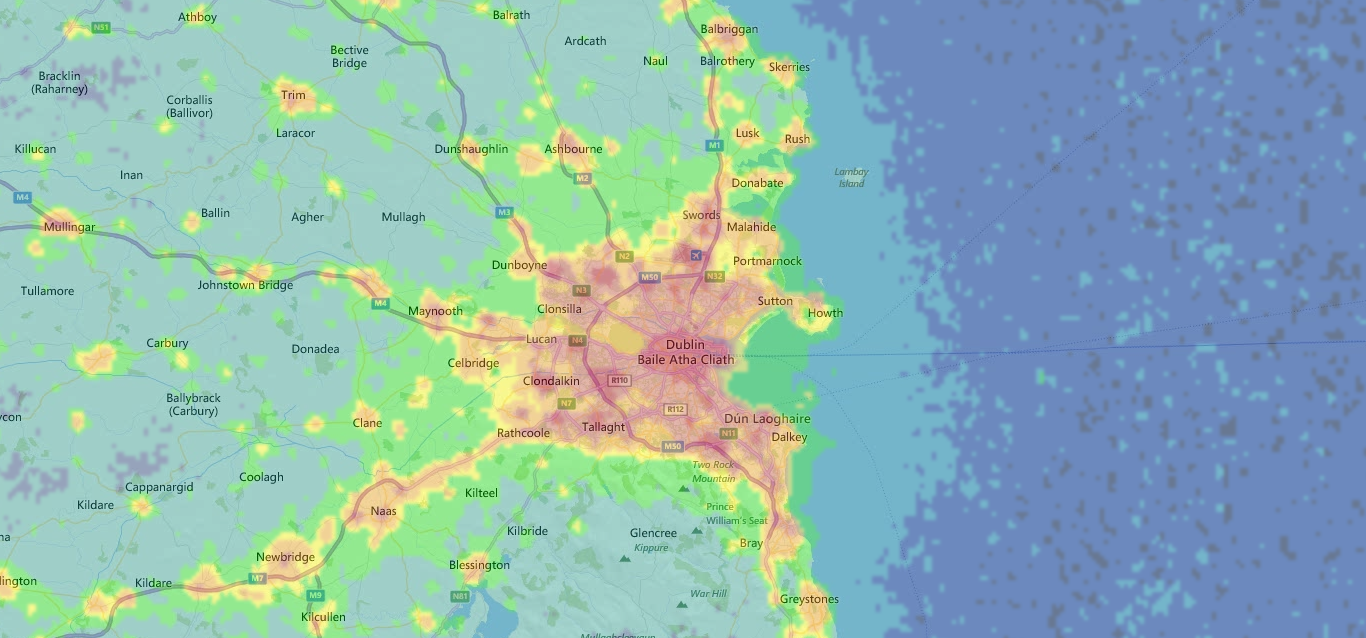
\includegraphics[width=\textwidth]{dublin}
        \caption{Nighttime Imagery of Dublin provided by the VIIRS 2018 (March) Radiance}
        \label{Dublin}
    \end{subfigure}
    \hfill
    \begin{subfigure}{.48\textwidth}
        \centering
        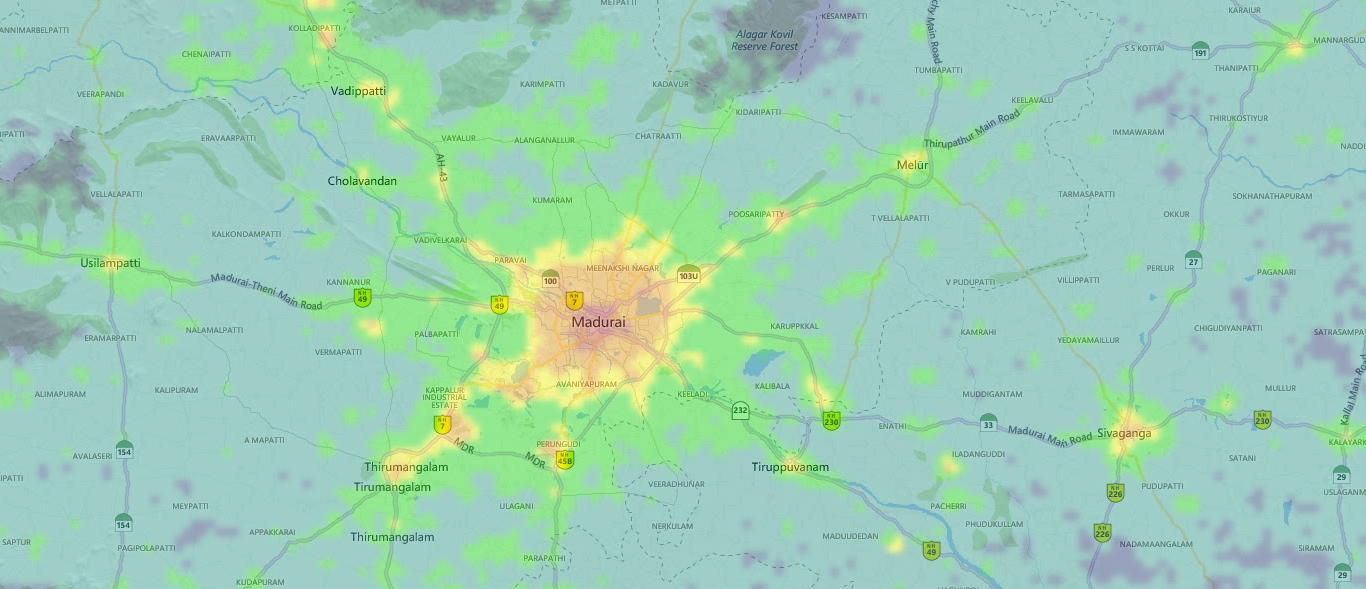
\includegraphics[width=\textwidth]{madurai}
        \caption{Nighttime Imagery of Madurai provided by the VIIRS 2018 (March) Radiance}
        \label{Madurai}
    \end{subfigure}
\end{figure}

However, Walker's Law predicts similar photopollution values in both scenarios. This is not the case, as is evident in figure \ref{fig:1}. Therefore, we can deductively conclude that the population density of an area is somehow related to the photopollution produced from that same area, and could be a better predictor of photopollution. 


\section{Hypothesis}
Our hypothesis says that a mathematical model can be created to predict photopollution in Munster based solely on population density. It assumes that population density is the main driving factor of photopollution and that all other factors are negligible. The independent variable in our case is population density and photopollution is the dependent variable.

\section{Experimental Method}
The experimental method being used to measure photopollution involves measuring the dark portion of the sky with a telescope and a photometer. Typically such measurements are made at the zenith: the point at which the sky or celestial sphere is directly above the observer.\cite{calculatelux}\cite{zenith} 
For our experiment, however, we will use a photometer app. We will use an app instead of a physical photometer as the photometer we bought proved to be incompatible with measuring through a telescope.

Measurements will be made at 20 sites located throughout Munster. These sites we plan on including are: Blackwater (Dark Site) (Kerry), Tipperary town (Tipperary), Cahir (Tipperary), Clonmel (Tipperary), Ballymacarbry (Waterford), Lismore (Waterford), Tallow (Waterford), Watergrasshill (Cork), Cork City (Cork), Macroom (Cork), Tarbert (Kerry), Kilrush (Clare), Ennis (Clare), Shannon (Clare), Limerick City (Limerick), Adare (Limerick), Newcastle West (Limerick), Tralee (Kerry), Killarney (Kerry), and Kenmare (Kerry). Population density for the different sites is provided by the Central Statistics Office.\cite{2016CensusTowns}\cite{2016ElectoralDiv}

Once all the data is collected, a relationship or trend in the data will be sought. This will be done with the help of a Python program Conor developed. We will also gather data about what the standard deviation in photopollution values is. The correlation coefficient will be used to see if there is a strong linear correlation in the data. Correlation coefficient is a measure of the strength of the linear relationship between to two sets of data. Correlation coefficient, r,  is a number in the following range: -1 $<=$ r $<=$ 1. If r is close to 1, then there is a strong positive correlation between the two sets of data. If r is close to -1, we say there is a strong negative correlation between the two sets. If r is close to 0, then there is no correlation between the two sets.\cite{am4}
The equation for the correlation coefficient is represented in the equation \ref{r}.\cite{r}

\begin{equation}
\label{r}
r = \frac{{}\sum_{i=1}^{n} (x_i - \overline{x})(y_i - \overline{y})}{\sqrt{\sum_{i=1}^{n} (x_i - \overline{x})^2(y_i - \overline{y})^2}} 
\end{equation}

We will also calculate the standard deviation. Standard deviation measures the average deviation or spread from the mean of all values in the data set. It is a reliable measure of spread, as it takes into account of all values in the set, unlike the range and interquartile range.
The equation for the standard deviation is represented in the equation \ref{stddev}.\cite{am4}

\begin{equation}
\label{stddev}
\sigma = \sqrt{\sum \frac{(x_i - \mu)^2}{n}} 
\end{equation}

\section{Ideal Outcomes}
If we are able to establish a relationship between the two variables, we will create a grading system that will determine what any photopollution value produced in any particular area would mean in relation to the stargazing conditions. Using this information, we will develop a Python program, and an app that will incorporate our model and grading system. Both applications will be published under the name Photopollution Calculator on Github, and the Google Play Store respectively.\cite{github}\cite{play_store} We will also develop a photopollution, and population density heat map of the Republic of Ireland using QGIS in order to compare them against nighttime imagery from VIIRS 2018 (March) Radiance.\cite{QGIS_software}\cite{VIIRS_compare} On each map, ROI was divided into the various electoral divisions (Electoral Boundaries were provided by the Central Statistics Office), and following which conditional formatting was used in QGIS to shade in the map.\cite{boundaries} The photopollution map was shaded based on the grading system we developed during this project.

This mathematical model proved to be reasonably accurate and could be used by amateur astronomers as a companion to a photopollution map to paint a better picture of the photopollution in the night sky. 
 

\chapter{Experimental Method} 
\section{Environmental Conditions}
The experiment was carried out between the 11th of November 2018 \& the 18th of November 2018. It was typically carried out between the hours of 18:00 \& 00:00. We collected this data during the winter time as the night sky emerges earlier in the evening. This experiment was carried out during the Moon's waxing crescent phase. This was done in order to avoid sky glow from the Moon artificially increasing the photopollution of the town. There was a little precipitation when we collected data from the town of Tipperary, however, the weather cleared up thereafter. It was important that this experiment was carried out in November rather then December, as the Christmas lights put up during the latter period would have also artificially increased the photopollution value. 

\section{Apparatus Used} 
\begin{itemize}
\item Celestron Astromaster 102AZ  with an aperture of 102 mm with 20 mm telescope eyepiece lens.\cite{telescope}
\item Smartphone with photometer app preinstalled (LUX Light Metre Pro).\cite{photometer}
\item Purple Toshiba Laptop running Ubuntu with the latest version of Python 2.7 installed. Python modules we utilised include: Pandas, Scipy, Numpy, and Mathplotlib. We used Python primarily for data analysis during this project.\cite{purple_toshiba}\cite{python}\cite{scipy}
\item QGIS for generating a photopollution map, and population density heat map.\cite{QGIS_software}
\item Renault Clio car used for traveling to all the great sites of Munster.\cite{fab}
\end{itemize}

\section{Labelled Diagram}
\begin{figure}[H]
    \centering
    \begin{subfigure}{.48\textwidth}
        \centering
        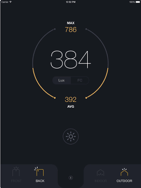
\includegraphics[width=\textwidth]{photometer}
        \caption{Photometer/LUX Light Metre}
    \end{subfigure}
    \hfill
    \begin{subfigure}{.48\textwidth}
        \centering
        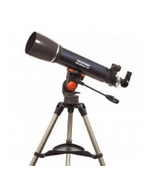
\includegraphics[width=\textwidth]{telescope}
        \caption{Telescope}
    \end{subfigure}
\end{figure}

\section{Procedure}  
\begin{enumerate}
\subsection{Data Collection}
\item We placed the telescope as close to the centre of the town as physically possible. (We used the same telescope eyepiece lens, photometer app and telescope throughout the experiment)
\item Once the telescope was set up, we placed the smartphone’s lens on the eyepiece lens of the telescope. We then opened the smartphone photometer application and prepared for recording the data.
\item We recorded our measurements with the telescope pointing towards zenith. This value is the photopollution produced by this particular area. We also recorded a maximum and minimum LUX value from that same portion of the sky.
\item We repeated Steps 1 - 4 at 20 different locations. We traveled to these sites using the fantastic Renault Clio, and included all the counties of Munster in this project.
\subsection{Data Analysis and Outcomes}
\item Once we collected all the data, it was time to find out whether there was a correlation between photopollution and population density. First, we visited the Central Statistics Office's website and downloaded a file containing the population density data for all the sites that we gathered data from.
\item Once we acquired this data, we inputted all the photopollution values collected using our photometer application into a Solver python program that Conor developed. This program printed all values inputted into it, found a correlation between the two variables, printed the correlation coefficient, standard deviation, and the equation describing the correlation. It also printed the correlation coefficient of Walker's Law, and outputted all the graphs that can be found throughout this Project Book. This was done using Mathpoltlib. (The code can be found in Appendices.)
\item Using this model, we were able to develop a grading system that can determine what any photopollution value produced in any particular area would mean in relation to the stargazing conditions. We did this by setting Limerick City as the baseline for terrible stargazing conditions (We choose Limerick City as, it was the site with the lowest population density that we deemed to be characterised with terrible stargazing conditions), and using this baseline we extrapolated five different grades for stargazing conditions, from excellent to terrible.  
\item Using the mathematical model and grading system, we generated a photopollution map using the software QGIS, and compared it against a nighttime survey of Ireland provided by the VIIRS 2018 (March) Radiance. 
\item Following which, Conor developed another Python program, and an app which incorporates our mathematical model and grading system to show the potential practical appliciations. This grading system took Limerick City as the base point for terrible stargazing conditions and giving a total of five different grades including terrible. (Code can be found in Appendices.)
\end{enumerate}






\chapter{Results}
\section{Scatter Plots}
\subsection{Scatter Plots of Our Main Results}
\begin{figure}[H]
    \centering
    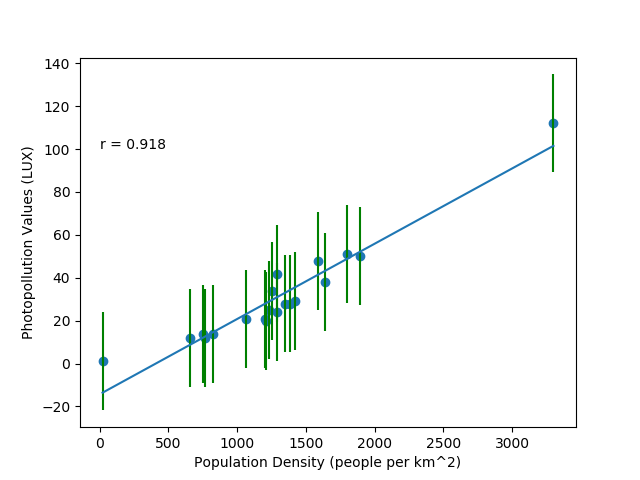
\includegraphics[width=.8\linewidth]{meanluxall}
    \caption{Mean Photopollution Values (All Sites)}
    \label{meanluxall}
\end{figure}
\begin{figure}[H]
    \centering
    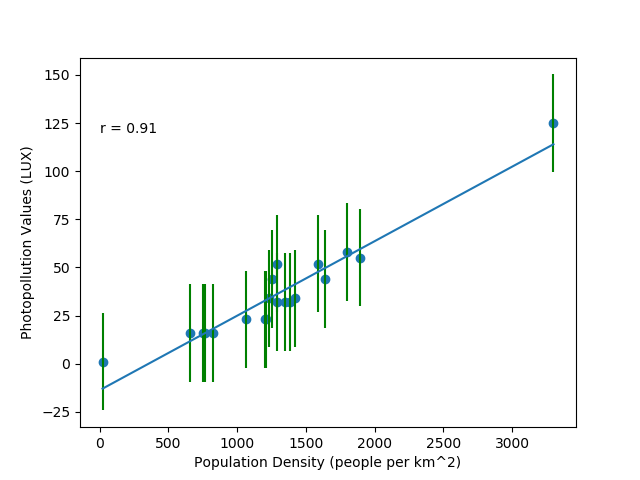
\includegraphics[width=.8\linewidth]{maxluxall}
    \caption{Max Photopollution Values (All Sites)}
    \label{maxluxall}
\end{figure}
\begin{figure}[H]
    \centering
    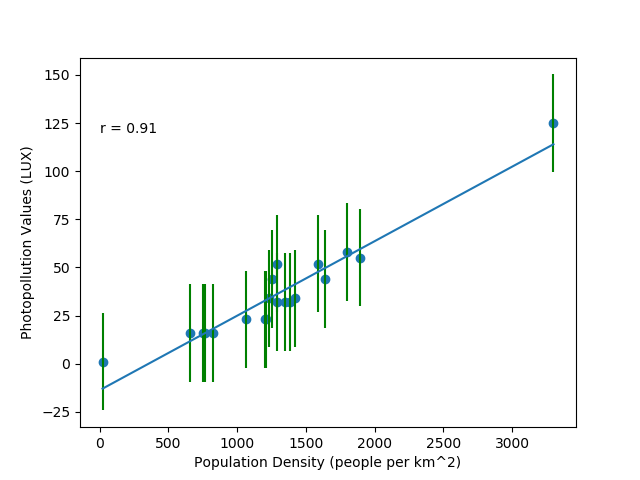
\includegraphics[width=.8\linewidth]{minluxall}
    \caption{Minimum Photopollution Values (All Sites)}
    \label{minluxall}
\end{figure}
\hfill
\subsection{Scatter Plots Based Results from Each County}
\begin{figure}[H]
    \centering
    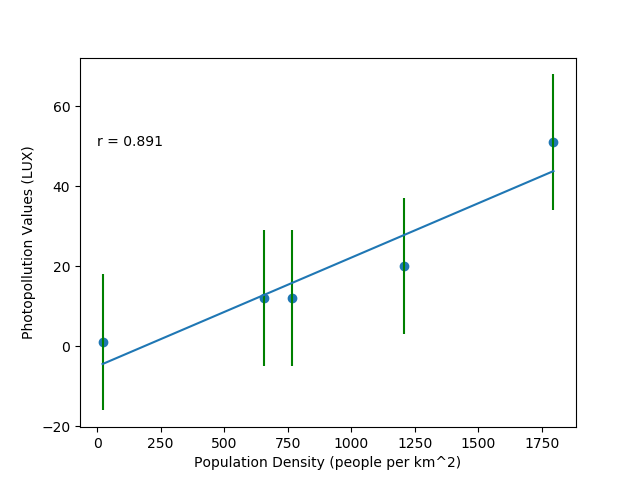
\includegraphics[width=.8\linewidth]{kerry}
    \caption{Kerry Photopollution Values}
    \label{kerry}
\end{figure}
\begin{figure}[H]
    \centering
    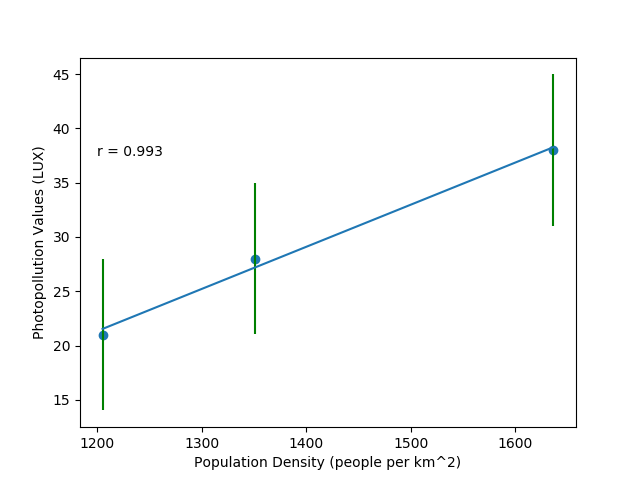
\includegraphics[width=.8\linewidth]{tipp}
    \caption{Tipperary Photopollution Values}
    \label{tipp}
\end{figure}
\hfill
\begin{figure}[H]
    \centering
    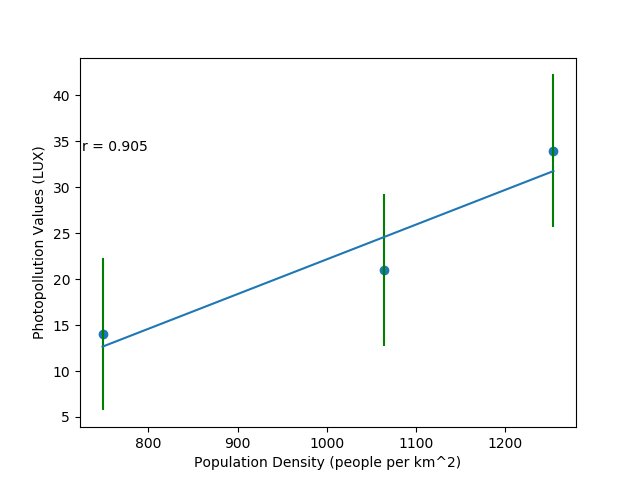
\includegraphics[width=.8\linewidth]{waterford}
    \caption{Waterford Photopollution Values}
    \label{waterford}
\end{figure}
\begin{figure}[H]
    \centering
    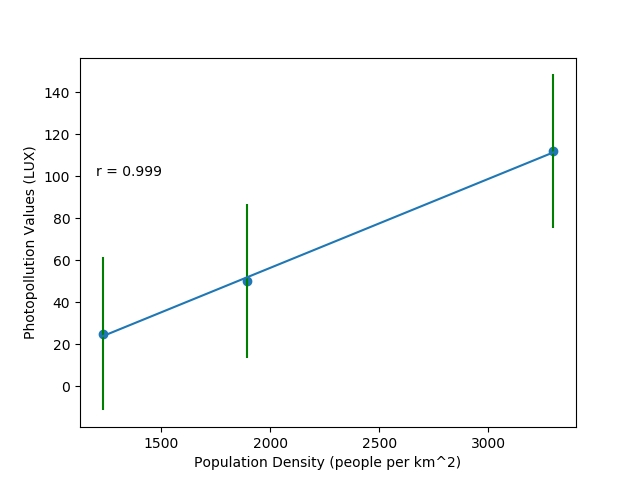
\includegraphics[width=.8\linewidth]{cork}
    \caption{Cork Photopollution Values}
    \label{cork}
\end{figure}
\hfill
\begin{figure}[H]
    \centering
    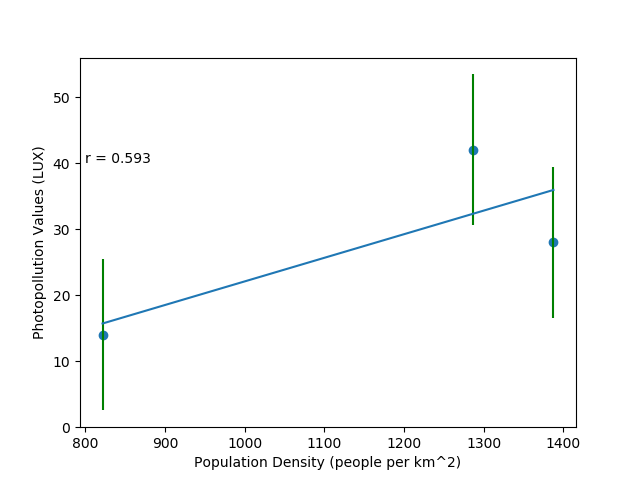
\includegraphics[width=.8\linewidth]{clare}
    \caption{Clare Photopollution Values}
    \label{clare}
\end{figure}
\begin{figure}[H]
    \centering
    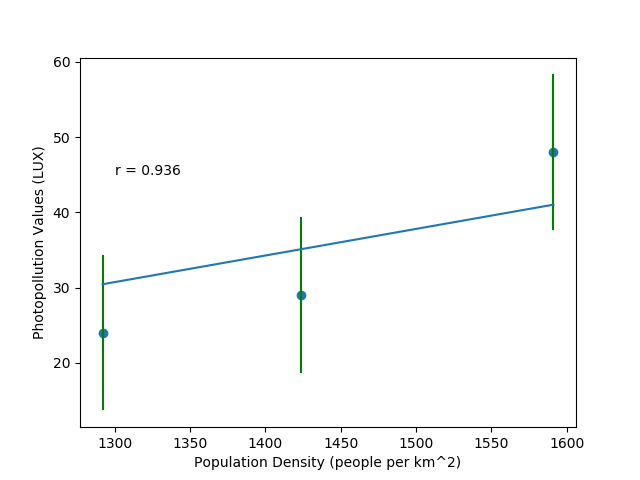
\includegraphics[width=.8\linewidth]{limerick}
    \caption{Limerick Photopollution Values}
    \label{limerick}
\end{figure}

\section{Mathematical Model}

\begin{equation}
\label{model} 
I = 0.03510566 d_x - 14.32414198 
\end{equation}

In this equation $I$ is the photopollution produced in that area, in the unit of measurement, $LUX$, and $d_x$ is the population density of that area (people per $km^{2}$). 

\hfill{}

\section{Grading System}
\begin{tabularx}{\textwidth}{|X|l|}
  \hline
  \textbf{LUX Value} & \textbf{Stargazing Conditions} \\ [25pt]
\hline
0 - 9 & Excellent Stargazing Conditions\\ [40pt]
\hline
9 - 17 & Good Stargazing Conditions\\ [40pt]
\hline
17 - 25 & Fair Stargazing Conditions\\ [40pt]
\hline
25 - 34 & Poor Stargazing Conditions\\ [40pt]
\hline
34 + & Terrible Stargazing Conditions\\ [40pt]
\hline
\end{tabularx}

\hfill

\section{Our Generated Maps}
\begin{figure}[H]
    \centering
    \caption{Maps generated in QGIS.}
    \label{qgis}
    \begin{subfigure}{\textwidth}
        \centering
        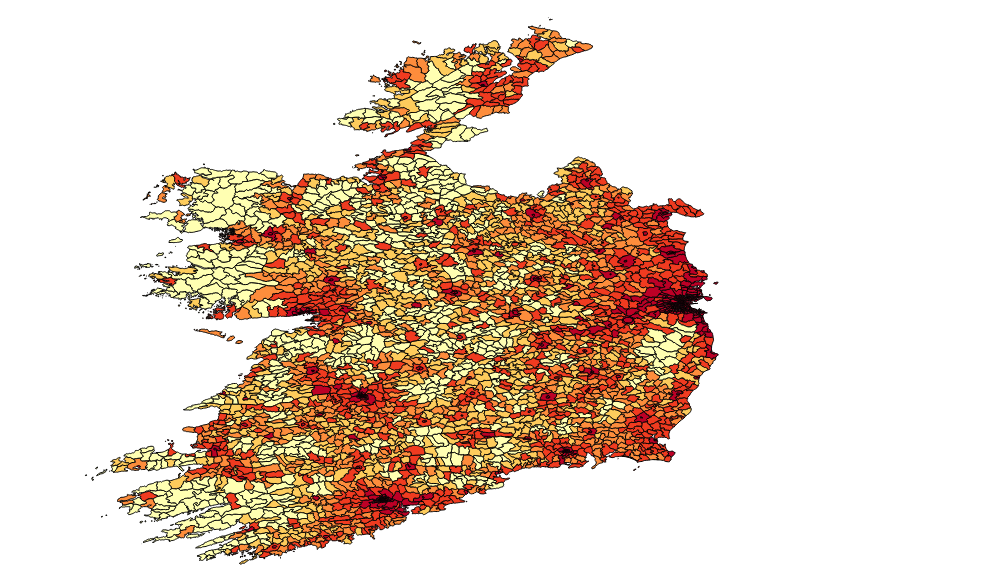
\includegraphics[width=\textwidth]{populationdensitymap}
        \caption{Our generated population density heat map of the Republic of Ireland}
        \label{pdheatmap}
    \end{subfigure}
    \hfill
    \begin{subfigure}{\textwidth}
        \centering
        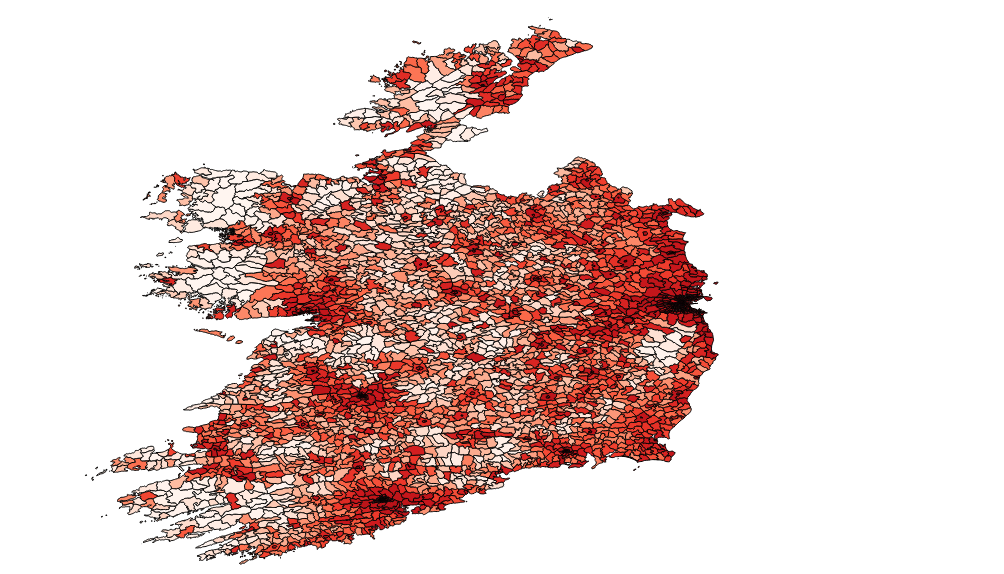
\includegraphics[width=\textwidth]{photopollutionmap}
        \caption{Our generated photopollution map of the Republic of Ireland}
        \label{photopollutionmap}
    \end{subfigure}
\end{figure}

\section{Nighttime Imagery of Ireland}
\begin{figure}[h]
    \centering
    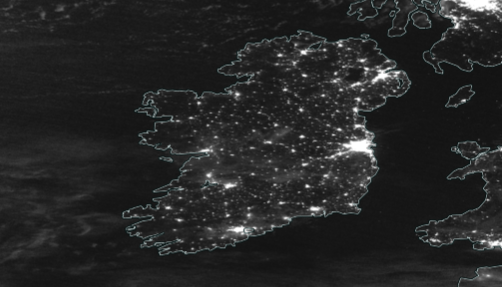
\includegraphics[width=\textwidth]{ireland}
    \caption{Nighttime Imagery of Ireland as provided by the VIIRS 2018 (March) Radiance.}
    \label{ireland}
\end{figure}

\chapter{Conclusions}
\section{Review of Results}
The aim of this project was to establish a mathematical model that could predict photopollution (the dependent variable) solely using population density (independent variable), and if we were able to create such a mathematical model, could we determine the severity of photopollution in each particular area.

Our findings suggests there is a relationship between the two variables. The relationship between the two variables is described in the equation \ref{modelrevisit}.

\begin{equation}
\label{modelrevisit}
    I = 0.03510413 d_x - 14.32180871 \tag{\ref{model} revisited}
\end{equation}

Therefore, we have an established an empirical relationship between the two variables. An empirical relationship is a relationship, or correlation that is supported by experiment and observation, but not necessarily supported by theory.\cite{empirical} The correlation coefficient is 0.916. Our correlation coefficient shows a strong positive correlation between photopollution and population density. This means that when population density increases, photopollution tends to increase. In comparison to Walker's law, we found a correlation coefficient of 0.61. Therefore, this suggests that there is a stronger correlation between population density and photopollution and that our findings support the conclusion that population density is a more reliable predictor of photopollution. Our findings can be summed up with figure \ref{qgis}, and figure \ref{ireland}. Figure \ref{pdheatmap}, is our generated population density heat map of Ireland, figure \ref{photopollutionmap}, is our generated photopollution map, and figure \ref{ireland} is a nighttime survey of Ireland. The figures are striking, and are practically identical. These figures beautiful prove our model's accuracy and the correlation between photopollution and population density. 

The mean of the photopollution value from all the data we collected was 31.2 LUX and the standard deviation was approximately 22.822. This suggests that a photopollution value below approximately 8.378 LUX, and above 54.022 LUX produced in a town is outside the norm. This is most likely an accurate representation of the photopollution produced in towns in the providence of Munster, as all towns in Munster fall between a population density of 600 and 2000 people per square kilometre (with the notable exception of Cork City). Therefore, we covered a wide spread of different values within this range. 

\section{Looking Back}
Looking back, while there may be a strong positive statistical correlation between the two variable, there is a few possible sources of error:

\begin{itemize}
\item The root of the equation \ref{modelrevisit} is at approximately 408.029416909. This means that this model is ineffective with population densities less than 409 people per $km^{2}$. A exponential equation would improve more effective, however, we did not have enough data to formulate such an equation.

\item While towns in Munster should have similar street lighting systems due to their close proximity, and their similar appearances on nighttime survey maps as provided by the VIIRS 2018 (March) Radiance, this does not necessarily mean these towns employ similar lighting systems.

\item During the data collection, the moon was gradually progressing towards a half moon. While this may not have had a large impact on the photopollution value collected from each site as the values were collected during the waxing crescent phase, there is certainly a possibly that it could have interfered slightly.

\item The weather in South Tipperary was partially cloudy. This could have possibly interfered with the measurements taken at the zenith at these locations. While weather was an issue in some instances, the days we chose, were the best possible days to carry out the experiment based on weather predictions from the astronomy forecast provided by Accuweather. 

\item The photometre app had a margin of error of approximately plus or minus five percent. While this is definitely not a terrible margin of error, there is certainly room for improvement. We did attempt to mitigate this error by using a handheld photometer, however, it proved to be incompatible for use with a telescope. The margin of error of said photometer, was approximately plus or minus 4 percent, therefore, possible changes in results would have been negligible.    

\item All population density data used throughout the course of this project was provided by the Central Statistics Office. Their latest population density figures were taken during the 2016 Census. Since 2016, population density figures of the sites we gathered data from could have deviated from their recorded values in 2016; therefore, this could slightly affect the accuracy and validity of our model. That being said, however, it has only been about two years since said Census, therefore, any changes in population density would be small, and as a result, would have a negligible impact on our results.

\item We cannot conclude that one of the variables is the cause of the other. A lurking variable, such as Gross Domestic Product, lighting systems, etc. could be responsible for the increase in photopollution (the dependent variable), i.e. \textbf{correlation does not always imply causality.}\cite{am4}
\end{itemize}

\section{Looking Ahead}
Looking ahead, there are a number of improvements we plan on implementing. 

\begin{itemize}
\item We would like to collect more data from various different sites, especially data that is currently on the extreme ends of our current sample set, i.e. population densities below 600 people per $km^{2}$, and above 2,000 people per $km^{2}$. We would also like to incorporate sites outside the providence of Munster, and when measuring new sites, we would like to use a photometer with an margin of error less than approximately plus or minus two percent. All of these additions would further test our model's accuracy, and will reduce the possible sources of error in our experimental method. This would also allow us to look into the possibility of an exponential equation better representing the relationship between photopollution and population density, as we would have a larger data set to deal with.  
\item As mentioned previously, all present models are currently based on Walker's Law, including fairly precise models, such as, Garstang’s Model.\cite{walkerlaw} These models make use what is called radiative transfer (the propagation of light rays through a medium together with absorption \& scattering). This can provide a more realistic model for areas close to the emitting source. However, in comparison to Walker's Law, we believe, and have shown that population density is a more reliable predictor of photopollution in any particular location. Therefore, we plan on incorporating various aspects of existing models, such as radiative transfer, into our model. We believe this would greatly enhance its accuracy, and vastly improve its ability to predict stargazing conditions accurately. 
\end{itemize}

\appendix
\appendixpage
\addcontentsline{toc}{chapter}{Appendices}
\begin{appendix}
\section*{Extra Scatter Plots}
\begin{figure}[H]
    \centering
    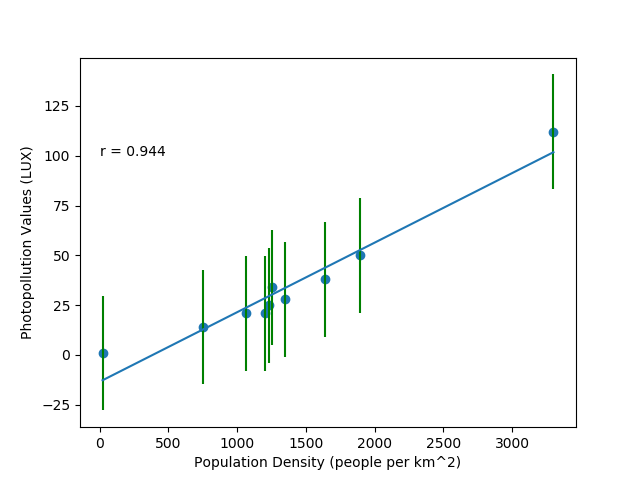
\includegraphics[width=.8\linewidth]{meanluxfirst}
    \caption{Mean Photopollution Values (First Site)}
    \label{meanluxfirst}
\end{figure}
\begin{figure}[H]
    \centering
    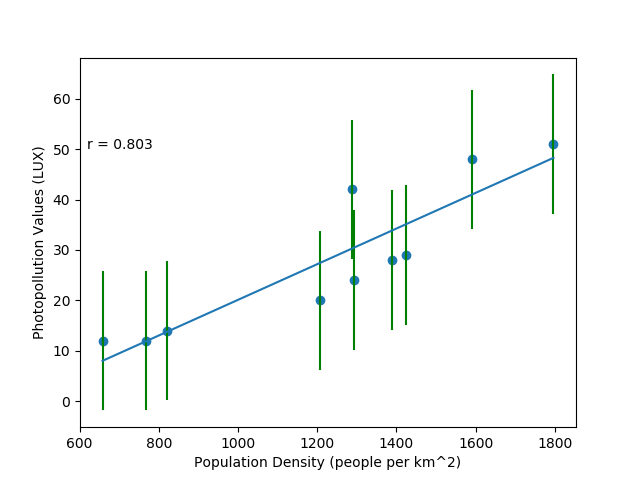
\includegraphics[width=.8\linewidth]{meanluxsecond}
    \caption{Mean Photopollution Values (Second Site)}
    \label{meanluxsecond}
\end{figure}

\newpage

\section*{Extra Table}
\begin{tabularx}{\textwidth}{|X|l|}
  \hline
  \textbf{The Name of the Site Visited} & \textbf{Mean Photopollution Value} \\ [15pt]
\hline
Blackwater Bridge (Dark Site) & 1 LUX \\ [15pt]
\hline
Tipperary Town & 21 LUX \\ [15pt]
\hline
Cahir & 28 LUX \\ [15pt]
\hline
Clonmel & 38 LUX \\ [15pt]
\hline
Ballymacarbry & 14 LUX \\ [15pt]
\hline
Lismore & 34 LUX \\ [15pt]
\hline
Tallow & 21 LUX \\ [15pt]
\hline
Watergrasshill & 50 LUX \\ [15pt]
\hline
Cork City & 112 LUX \\ [15pt]
\hline
Macroom & 25 LUX \\ [15pt]
\hline
Tarbert & 12 LUX \\ [15pt]
\hline
Kilrush & 14 LUX \\ [15pt]
\hline
Ennis & 42 LUX \\ [15pt]
\hline
Shannon & 28 LUX \\ [15pt]
\hline
Limerick City & 47 LUX \\ [15pt]
\hline
Adare & 24 LUX \\ [15pt]
\hline
Newcastle West & 29 LUX \\ [15pt]
\hline
Tralee & 20 LUX \\ [15pt]
\hline
Killarney & 51 LUX \\ [15pt]
\hline
Kenmare & 12 LUX \\ [15pt]
\hline
\end{tabularx}

\newpage

\section*{Python Programs}
\subsection*{Solver Program}
\lstinputlisting[language=Python, breaklines=true]{Python_Code_for_LaTex/Solver.py}

\hfill

\subsubsection*{Main Program}
\lstinputlisting[language=Python, breaklines=true]{Python_Code_for_LaTex/Program.py}

\section*{Email Correspondences with Prof. Brian Espey}

\author{Conor Casey \\ email \href{mailto:16ccasey@student.kenmarecs.com}{16ccasey@student.kenmarecs.com} 
   \and Prof. Brian Espey \\ email \href{mailto:someone@somewhere.com}{someone@somewhere.com} 
}

\textbf{From: Conor Casey, To: Prof. Brian Espey}

I am doing a project called “Is It Possible to Create a Mathematical Model to Predict Photopollution Based on Population Density in Munster” for the BTYSTE 2019.
I am contacting you to enquire if you would be willing to answer some questions on light pollution. The answers to these questions would be included in my Project Book. 


\textbf{From: Prof. Brian Espey, To: Conor Casey}

Hi Conor,

Sure- send the questions on. I presume that you've done some research and come across the Walker model for light pollution? see, e.g. adsbit.harvard.edu/cgi-b...e=.pdf

Best regards,

Brian.



\textbf{From: Conor Casey, To: Prof. Brian Espey}

Professor Espey,
Thank you for responding to my email. It is greatly appreciated.
I had not previously seen this particular paper before, however, I am familiar with the Walker model.
I have a number of questions to ask you:

1)  What equipment/apparatus did you use to carry out your observations for Light Pollution in the Irish Context.

2)  You make reference several times in your research to the comparison between Northern Ireland and the Republic in terms of light pollution? Did you make any measurements in Northern Ireland and if so how many and at what sites?

3) Do you think the unit LUX is an appropriate unit of measurement for photopollution?

4) Could population density be a lurking variable in the Walker Model? As in, due to the fact that population density decreases with an  increased distance from the city centre (CBD), could population density actually be responsible as opposed to distance and population size. I have attached a link discussing the relationship between population and distance from the central business district in relation to population size:
adsbit.harvard.edu/cgi-b...e=.pdf

5) Why in the Walker Model, $\frac{mag}{sec^{2}}$ is the unit of measurement used?

I also wanted to enquire if the Trinity Physics Department would be willing to take Transition Year students for work experience, if so who should I contact.


\textbf{From: Professor Brian Espey, To: Conor Casey}

Hello Conor,

See the text below each question for answers.

Hope this helps- let me know if you have more questions.

Brian.

\textbf{Answers:}

I have used a combination of the Sky Quality Meter equipment

(www.unihedron.com) in both the hand-held SQM, SQM-L models and also the datalogging equipment. I have also used a modified version as described in  

journals.sagepub.com/doi/abs/10.1177/1477153513515508.
I have data for a number of sites in Northern Ireland, but the quotes refer to measurements of the light emitted from the Republic \& Northern Ireland as seen by satellites.

Population density may come into play as putting everyone in apartment blocks would lead to a different number of streetlights than if they all lived in semi-detached or terraced houses, for instance, but the smooth fall-off in light with distance from Dublin City Centre, for instance, shows that the light from many locations is combined, so it's not simply a case of being due to the local population density, otherwise the light would fall off much more strongly when outside the city limits. The light falling on an area is due to the combination of a range of locations, so is probably more closely related to the overall population than the local population density, though the relative importance of each is something I hope to work on further.

Magnitudes are an old astronomy unit, so mpsa units are used as the SQM was developed for astronomers

We don't have placements per se at the moment, but there are TY experience days and your school science teacher should have received information. If not, contact: Helen O'Hallhoran at: hohllorn@tcd.ie


\textbf{From: Conor Casey, To: Professor Brian Espey}

Professor Espey,
Thank you so much for these very comprehensive answers. I just have two more questions if you don’t mind me asking:

1) In relation to the Walker Model, does the model still apply in situations where there are two major urban population centres next to each other, like for example in the case of Liverpool and Manchester?

2) In your experience and results, has the Walker model been a reliable predictor of light pollution?

Thank you again for answering my questions, it is greatly appreciated. I will send you the results and Project Book for my BT project once everything is put together, if you are interested.

Kind Regards,

Conor.


\textbf{From: Professor Brian Espey, To: Conor Casey}

Sorry for the delay, Conor, as we've had exams (and marking!) recently. Your question got me thinking, so I pulled out some data to see how well it fits the Walker model- I should have results back to you later today.

I hope that the delay hasn't held you up too much. One question: are you going to model the light in Munster, or is this purely a review of the light pollution modelling approaches? The Walker (and Garstang) models have been used in various guises (and with improvements) over the years, but the basic idea that it's possible to model light pollution probably stems from these two main works.

Regards,

Brian.


\textbf{From: Professor Brian Espey, To: Conor Casey}

Hello again Conor, and apologies for the delay in replying.

Yes, I believe that the Walker model will apply as well even for connurbations close to each other, but recall that the model in its simplest form pictures the town or city as a point source, so the effect of combinations would be best modelled by this method when the distance from the centre of mass of the combination is at least several times the separation from each other. 

I looked at some data I have for Dublin and Galway and find that the variation in sky brightness with distance is broadly similar, but differs from the simple Walker model - I get between -0.5 (for Galway) and -1.25 (for Dublin): for both these cases I've looked at data from just outside the city outwards.

In terms of accuracy, models have grown more complicated and are, as I noted before, based on Garstang models as well. These models make use what is called radiative transfer (the propagation of light rays through a medium together with absorption \& scattering) - see, for instance the reference to Berry's modelling approach, or the Polish work, which uses satellite data to provide the light emission intensity and distribution used for the model (the VIIRS data in the lightpollutionmap linked below), and the effect of shadowing by higher ground etc, and which can also provide a more realistic model for areas close to the emitting source. See: https://w1.cegepsherbrooke.qc.ca/~aubema/LPTMM//uploads/Site/modelling-netzel.pdf

Is this what you need? I don't want to overload you, but if you're doing a simple model you can take the town populations and make a simple Walker model and see how you do and compare the result with the atlas data at:

https://www.lightpollutionmap.info/\#zoom=9\&lat=6800983\&lon=-974765\&layers=0BFFF
FTFFFT

Brian.
\end{appendix}

\printbibliography[heading = bibintoc]

\end{document}